\documentclass[english,twoside,censored,tkt]{HYthesisML}

\PassOptionsToClass{openany,twoside,a4paper}{report}

\usepackage{csquotes}
\usepackage[style=authoryear,bibstyle=authoryear,backend=biber,natbib=true,maxnames=99,maxcitenames=2,uniquelist=minyear,giveninits=true,uniquename=mininit]{biblatex}
%\usepackage[style=numeric,bibstyle=numeric,backend=biber,natbib=true,maxbibnames=99,giveninits=true,uniquename=init]{biblatex}

\addbibresource{bibliography.bib}
\DeclareNameAlias{sortname}{family-given}

\usepackage[utf8]{inputenc} % For UTF8 support, in some systems. Use UTF8 when saving your file.

\usepackage{xr-hyper}
\usepackage{amsthm}
\usepackage{lmodern}         % Font package, again in some systems.
\usepackage{textcomp}        % Package for special symbols
\usepackage{float}
\usepackage[pdftex]{color, graphicx} % For pdf output and jpg/png graphics
\usepackage{epsfig}
\usepackage[pdftex, plainpages=false]{hyperref} % For hyperlinks and pdf metadata
\usepackage{fancyhdr}        % For nicer page headers
\usepackage{tikz}            % For making vector graphics (hard to learn but powerful)
\usepackage{amsmath, amssymb} % For better math
\usepackage{subcaption}

\singlespacing               %line spacing options; normally use single

\graphicspath{{./images}}
\fussy
\overfullrule=1mm


\title{TBD}
\author{Viktor Horsmanheimo}
\date{\today}

\supervisors{Mohamed Taoufiq Damir}

\keywords{FPGA, cryptography}
\additionalinformation{\translate{\track}}

%% Provide classification terms, to appear on the abstract page.
%% Replace the classification terms below with the ones that match your work.
%% ACM Digital library provides a taxonomy and a tool for classification
%% in computer science. Use 1-3 paths, and use right arrows between the
%% about three levels in the path; each path requires a new line.

\classification{\protect{\ \\
\  General and reference $\rightarrow$ Document types  $\rightarrow$ Surveys and overviews\  \\
\  Applied computing  $\rightarrow$ Document management and text processing  $\rightarrow$ Document management $\rightarrow$ Text editing
}}

%% If you want to quote someone special. You can comment this line out and there will be nothing on the document.
%\quoting{Bachelor's degrees make pretty good placemats if you get them laminated.}{Jeph Jacques}


%% OPTIONAL STEP: Set up properties and metadata for the pdf file that pdfLaTeX makes.
%% Your name, work title, and keywords are recommended.
\hypersetup{
    unicode=true,           % to show non-Latin characters in Acrobat’s bookmarks
    pdftoolbar=true,        % show Acrobat’s toolbar
    pdfmenubar=true,        % show Acrobat’s menu
    pdffitwindow=false,     % window fit to page when opened
    pdfstartview={FitH},    % fits the width of the page to the window
    pdftitle={TBD},            % title
    pdfauthor={Viktor Horsmanheimo},           % author
    pdfsubject={FPGA uses in cryptography},          % subject of the document
    pdfcreator={Viktor Horsmanheimo},          % creator of the document
    pdfproducer={pdfLaTeX}, % producer of the document
    pdfkeywords={something} {something else}, % list of keywords for
    pdfnewwindow=true,      % links in new window
    colorlinks=true,        % false: boxed links; true: colored links
    linkcolor=black,        % color of internal links
    citecolor=black,        % color of links to bibliography
    filecolor=magenta,      % color of file links
    urlcolor=cyan           % color of external links
}

%%-----------------------------------------------------------------------------------

% Theorems
\theoremstyle{definition}
\newtheorem{definition}{Definition}[section]
\newtheorem{example}{Example}[section]

\begin{document}

% Generate title page.
\maketitle

%%%%%%%%%%%%%%%%%%%%%%%%%%%%%%%%%%%%%%%%%%%%%%%%%%%%%%%%%
%% STEP 3:
%%%%%%%%%%%%%%%%%%%%%%%%%%%%%%%%%%%%%%%%%%%%%%%%%%%%%%%%%
%% Write your abstract in the separate file, to be positioned here.
%% You can make several abstract pages (if you want it in different languages),
%% in which case you should also define the language of the abstract,
%% as below.

\begin{abstract}
Write your abstract here.

In addition, make sure that all the entries in this form are completed.

Finally, specify 1--3 ACM Computing Classification System (CCS) topics, as per \url{https://dl.acm.org/ccs}.
Each topic is specified with one path, as shown in the example below, and elements of the path separated with an arrow.
Emphasis of each element individually can be indicated
by the use of bold face for high importance or italics for intermediate
level.

\end{abstract}


% Place ToC
%\newpage
\mytableofcontents

\mainmatter

\chapter{Introduction\label{intro}}

\textit{Field Programmable Gate Arrays} (FPGA) are chips that unlike standard
ones such as CPUs, are programmable after manufacturing. Because of this they
have become increasingly more popular in the past few decades. FPGAs consist of
logic gate arrays which in theory can evaluate any boolean function. In this
thesis we will give an overview on FPGAs with a focus on cryptography.

FPGAs were developed in the 80s by Altera, at that time they were not very
practical due to the size of the transistors being very large. This meant that
a chip could not fit many transistors and were limited in what they could do.
Moore's law states that the transistor size halves every two years, this has
affected FPGAs as well and they now contain enough transistors to compete with
\textit{Application Specific Integrated Circuits} (ASIC). An ASIC is a type of
hardware that is made specifically for a task, for example cryptographic
currency mining hardware. These chips are in general faster and use less energy
than FPGAs if the manufacturer is working with the latest technology. ASICs are
costly, if anything goes wrong after production it is extremely expensive to
rectify such a mistake. This is where FPGAs are very useful as they are
reprogrammable, ASICs can be first implemented on an FPGA. Once the chip has
been verified that it works, it can be ported to an ASIC. This minimizes the
amount of bugs found after the ASIC is manufactured.

\section{Outline\label{outline}}
In Chapter \ref{FPGA} we will go into detail about how FPGAs work internally,
how they are configured and the technologies behind it. In Chapter \ref{crypto}
we will give an overview about symmetric, asymmetric cryptography and how
reconfigurable hardware can be used with it.

\chapter{FPGA\label{FPGA}}
As briefly mentioned in the introduction, FPGAs consisting of an array of logic
gates. In this section we will give an overview about how they and other the
other components work and what different ways there are to configure these
chips. Modern FPGAs may also include a number of other components, for example
processors and multipliers though we will not cover those.

\section{Components}
\subsection{Lookup tables}

In boolean algebra we can represent a function as a truth table of size $2^N$
where $N$ is the amount of variables in the function. This translates directly
to binary and because of this property FPGAs extensively use lookup
tables(LUT). The way LUTs are implemented are using $N:1$ multiplexers and
$N$-bits of memory, it stores all the answers of the LUT in memory. Then the
multiplexer takes $N$ inputs and maps it to the LUTs answer. For example if we
have the following function.

$$A + B \times C$$

There are $2^3 = 8$ different answers to the function. We then
store all of these answers in memory in a table as similar to what is seen in
table \ref{tab:example_truth_table}.

\begin{table}[ht]
    \centering
    \begin{tabular}{|l|l|l|l|}
        \hline
        A & B & C & Out \\ \hline
        0 & 0 & 0 & 0   \\ \hline
        0 & 0 & 1 & 1   \\ \hline
        0 & 1 & 0 & 0   \\ \hline
        0 & 1 & 1 & 1   \\ \hline
        1 & 0 & 0 & 0   \\ \hline
        1 & 0 & 1 & 1   \\ \hline
        1 & 1 & 0 & 1   \\ \hline
        1 & 1 & 1 & 1   \\ \hline
    \end{tabular}
    \caption{Example truth table}
    \label{tab:example_truth_table}
\end{table}

% flip flops
This alone isn't enough to be able to implement everything as we cannot store
state. What we need is some way to store information, this is where delay(D)
flip-flops come in. Here we have an example of how an FPGA might use a
flip-flop as seen in Figure \ref{fig:lut_flipflop}. They can store a single bit of data, with
this the chip can store state and is now complete.

\begin{figure}[H]
    \centering
    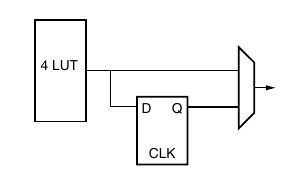
\includegraphics[scale=0.6]{lookup_table_flipflop.png}
    \caption{An example of how a lookup table could be implemented \cite{m_d_mano_digital_2012}}
    \label{fig:lut_flipflop}
\end{figure}

These LUTs are what allow for FPGAs to be reconfigured. By simply writing to
the tables the correct values it allows the chip to implement any function.
There's been studies done about how many LUTs a logic block should contain, if
there were more LUTs it would allow for more complex logic. Though adding more
inputs would also make the chip slower \cite{amano_principles_2018}.

\begin{figure}[H]
    \centering
    \label{fig:fpga_structure}
    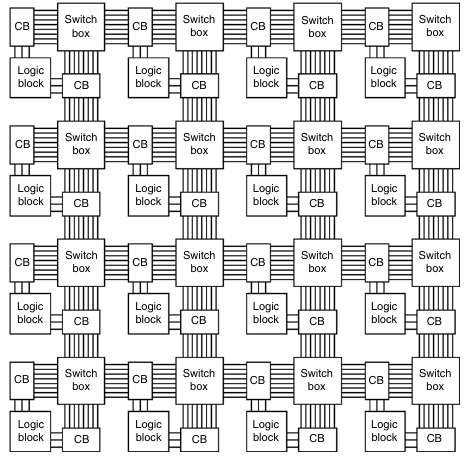
\includegraphics[scale=0.7]{fpga_structure.png}
    \caption{An example of an island-style FPGA\cite{m_d_mano_digital_2012}}
\end{figure}

\subsection{Input/Output blocks}
Input/Output blocks (I/O blocks, IOB) are blocks that are placed around the
periphery of the FPGA. They control the interface between the FPGA and external
circuits such as the clock and power usage.

\subsection{Connection block}
Along the wires by the logic blocks there are connection blocks (CB). These blocks
control which data goes into and out of a logic block. They also connect the
I/O blocks to the FPGA.

\subsection{Switch block}
A switch block (switch box, SB) is a type of block that exists at every
intersection in the wiring. As the name suggests it's built from a bunch of
switches and it's job is to route the electricity between the logic blocks.
There are different types of implementations for switch blocks, depending on
the type it will have different levels of connectivity and efficiency. Though
the specifics of this is out of the scope of this paper.

\subsection{Connections}
There are multiple ways the logic blocks can be connected, Xilinx FPGAs have
four different types of interconnects: long lines, hex lines, double lines and
direct lines. The direct lines are to connect neighboring logic gates for fast
transfer. Hex and double lines connect logic gates that are a medium length
away. Long lines go along the entire chip and are often used for signals that
everything needs to know.


\section{Configuration}
There are various ways reprogrammability can be implemented, though we're only
going to focus on the three main technologies: static RAM, flash memory and
antifuse.

\subsection{Static RAM}
Static RAM, or SRAM is a very common way to handle configuration. It's great
because it is fast and has infinite reconfiguration. The issues with SRAM is
that it's volatile which means that if power is lost so is the configuration.
Another issue is power consumption, as the SRAM cell contains 6-12 transistors
compared to flash memory which only requires roughly two transistors
\cite{amano_principles_2018}.

\subsection{Flash memory}
Flash memory is a way to store the configuration in memory without needing
power for the chip to remember it. It works by having electrically erasable
programmable read-only memory, it's benefit is that the configuration can be
remembered even if the device is powered off. The downside is that there's only
a limited amount of writes before it fails and that flash is often slower at
writing than SRAM \cite{m_d_mano_digital_2012}.

\subsection{Antifuse}
An antifuse is the opposite of a fuse, it works by having high resistance and
not allowing electricity to pass until the fuse is blown. This technology is
very reliable and rarely corrupts, which is why it's often used in places with
for example radiation. The down side of antifuses is that it can only be
programmed once, after it's programmed the fuses are blown and can not be
restored.

\chapter{Cryptography\label{crypto}}
Cryptography has always been important, it's been used since ancient times to
secure communication. In today's world where we have a lot of information that
needs to get from place to place it is especially important to make sure that
it isn't tampered with. We have lots of ways to make sure that it gets
transported safely, in this chapter we're going to give an overview about
different kinds of cryptography and how it can be used in junction with FPGAs.
FPGAs can make for example hash functions among other things faster. With
quantum computers coming soon the cryptographic functions we have now, for
example RSA can be broken in polynomial time.

\section{Public key cryptography}
Public key cryptography is works by having having two sets of public- and
private keys. Before the 1976 public key cryptography was quite difficult there
were no good way to exchange keys. This changed when the Diffie and Hellman key
exchange was invented \citep{FranciscoRodriguez-Henriquez10}. This allowed for
keys to be exchanged quickly and securely.



\chapter{Conclusions\label{conclusions}}


\addcontentsline{toc}{chapter}{\bibname}
\printbibliography

%%%%%%%%%%%%%%%%%%%%%%%%%%%%%%%%%%%%%%%%%%%%%%%%%%%%%%%%%
\backmatter
\begin{appendices}

%% A sample Appendix

\appendix{Sample Appendix\label{appendix:sample}}

You can add one or more appendices to your thesis.

\end{appendices}
%%%%%%%%%%%%%%%%%%%%%%%%%%%%%%%%%%%%%%%%%%%%%%%%%%%%%%%%%

\end{document}
